\documentclass[a4paper,11pt]{article}
\usepackage[english]{babel}
\usepackage[utf8]{inputenc}
\usepackage[T1]{fontenc}
\usepackage{times}
\usepackage{lastpage}
%\setcounter{secnumdepth}{0} %To remove section numbering.
\usepackage[margin=3cm, vmargin={100pt,100pt}]{geometry}
\usepackage{fancyvrb}
\usepackage{graphicx}
\usepackage{listings}
\usepackage{amsfonts}
\usepackage{amsmath}
\usepackage{url}
%\usepackage{draftwatermark} %To mark as draft.

\newcommand{\footnoteremember}[2]{
\footnote{#2}
\newcounter{#1}
\setcounter{#1}{\value{footnote}}
}
\newcommand{\footnoterecall}[1]{
\footnotemark[\value{#1}]
}

\title{Leversi}
\author{Linus Närvä (c10lna)}

\begin{document}
\maketitle

\begin{tabular}{l l}
Course: & Artificial Intelligence - Methods and Applications (Fall 14) \\
Teachers: & Ola Ringdahl, Juan Carlos Nieves Sanchez \\
Institution: & Computer Science \\
\end{tabular}

\section{Introduction}
This report describes the implementation of Leversi. A Reversi game implementation with a graphical user interface. The focus of this report lies on the implementation of the AI player.

\subsection{Work in progress}
At the time of writing, the GUI part of the program is not yet finished.

\section{Implementation details}
Everything was implemented in c++11 using the Gtkmm package to implement the GUI parts. It is intended to run on Linux, so in the getting started section the operating system is assumed to be Linux.

\section{Getting started}
The first thing to do is of course to download the file. It can be found in the Umeå University CS department computer system at:
\begin{quotation}
\url{~c10lna/edu/5DV122/lab1/leversi}
\end{quotation}

\subsection{Requirements}
g++4.8 or later and gtkmm 3.0 or later.

\subsection{Compilation}
Just enter the directory 'src' and run \textit{make build}\footnote{Just running \textit{make} will also attempt to compile the unit tests which adds the unit test framework 'Catch 1.0' to the dependencies.}. Then run \textit{make purge} to remove object files and unit test files (optional). This should create two executables. \textit{leversi} and \textit{leversi-bot}. The former runs the program with the GUI. The second is a command line interface for reading in a state representation and return a move.

\subsection{Execution}
\subsubsection{leversi}
Make sure that the the directory you run it from includes the \textit{res} directory (containing the graphical objects used). Then just run the executable.

\subsubsection{leversi-bot}
Run the executable with no arguments and it will print usage information to standard error.

\section{Game representation}
The class representation of the game model are described in table \ref{tab:model}.

\begin{table}

\centering
\begin{tabular}{|l|p{12 cm}|}
\hline
\textbf{class} & \textbf{description}
\\ \hline
ReversiState & State representation with getters and setters for all values. It is not responsible for keeping itself legal, and does not implement any portion of the transition model.
\\ \hline
ReversiAction & Defines the transition model i.e. moving from one state to another, by applying an action and without breaking any rules.
\\ \hline
Outcome & Trivial but important class specifying the outcome of an action after it has been applied (sufficient information to undo the action to restore the state). It is implemented as a struct containing the action and the flips it caused.
\\ \hline
Game & The full game is all events that happened during the play. It is implemented as a \textit{current state} and a list of outcomes of actions. Actions can be \textit{committed} to the game, modifying the state and adding the outcome to the history. Actions can also be undone, restoring an earlier state of the game.
\\ \hline
\end{tabular}

\caption{Describes the most significant class components of the Reversi game model.} \label{tab:model}

\end{table}

The most significant part of of this model implementation is the class \textit{Game}. It stores only one copy of ReversiState in memory, but allows actions executed on this state to be undone. Intuitively this should yield better performance during maximin search, because the state doesn't need to be copied in recursive calls. Only one state representation is ever stored in memory.

\section{Decision procedure}
The desicion procedure for choosing the move is divided over three logical components. The \textit{move searcher} (MaximinSearcher) searches for a move that is in some sense optimal. The \textit{evaluator} (WashingtonEvaluator.hpp) evaluates a states and moves, thus defining what is considered optimal by the move searcher. Finally the \textit{time manager} ensures that maximum performance is obtained, given a tolerated \textit{latency}.

\subsection{Searching for the best move}
The \textit{move searcher} uses the method of \textit{maximin adversial search}, with \textit{alpha-beta pruning} and \textit{move ordering}. The original Maximin adversial search algorithm is used (as described in figure 5.7 on page 170 of \cite{aibook}), with one minor modification. $Max-Value$ and $Min-Value$ are not responsible for termination detection. Instead an intermediate recursive call handles termination detection and also move ordering. The relevant member functions of MaximinSearcher are described in table \ref{tab:maximinfunc}.

\begin{table}

\centering
\begin{tabular}{|l|p{12 cm}|}
\hline
\textbf{member function} & \textbf{description}
\\\hline
$maximinAction()$ & A user friendly interface omitting the recursion stuff. Just calls $\_maximinAction()$ with initial parameters.
\\ \hline
$\_maximinAction()$ & Recursive sub function. Performs termination detection and move ordering. Calls $maxValue()$ or $minValue()$ depending on if the max or minplayer are currently playing in the state.
\\ \hline
$maxValue()$ & Expands a max node. Calls $\_maximinAction()$.
\\ \hline
$minValue()$ & Expands a min node. Calls $\_maximinAction()$.
\\ \hline
\end{tabular}

\caption{Table summarising the \emph{MaximinSearcher} member functions responsible for the search, and how they relate to each other. It is somewhat simplified.} \label{tab:maximinfunc}

\end{table}

\subsection{State evaluation}
Two evaluators are have been implemented. SimpleEvaluator is the simplest evaluator possible. Its utility function just computes
\begin{quotation}
$utility :=  numMaxCoins - numMinCoins$. 
\end{quotation}
The more sophisticated utility implemented as the WashingtonEvaluator class (it is called WashingtonEvaluator because it was invented at Washington university). Basically it does four things.
\begin{enumerate}
\item Tries to maximise the number of coins.
\item Tries to minimize the mobility of the opponent.
\item Tries to grab the corners.
\item Tries to grab 'stable' positions, which are less likely to be taken later in the game.
\end{enumerate}
See the article\cite{utility} for details.

The evaluator is also responsible for computing a move utility score used for move ordering. This score does not take into account if the min or max player is playing (The zero-sum rule says that ``what the min player gains what the max player looses''). The implementation is trivial and just computes the gain of advantage in number of coins by the player compared to the adversary. The formula is
\begin{quotation}
\begin{tabular}{l l}
$moveUtility := 1 + 2*numFlips$, & or just \\

$moveUtility := 0$ & if the action was \textit{pass}.
\end{tabular}
\end{quotation}
The WashingtonEvaluator inherits this utility from SimpleEvaluator.

%\subsubsection{Algorithm descriptions}
%\begin{lstlisting}
%FUNCTION maximinAction(alpha, beta, depth) -> <OhelloAction, Score>
%BEGIN
%
%	IF depth => maxDepth OR gameOverCriteria() THEN
%	
%		score := utility(state)
%		action := createDummyAction()
%
%		RETURN <action, score>
%		
%	ENDIF
%	
%	% Placements only, not pass. Outcomes are typles of actions and
%	% flips they cause.
%	outcomes := findLegalPlacements(state)
%
%	IF outcomes.isEmpy() THEN
%		passAction = ReversiAction::pass()
%		passScore := evaluator.evaluate(passAction)
%		outcomes.insert(<passAction, passScore>)
%	ENDIF
%	
%	% Ranked actions contains an ordered set of actions.
%	rankedActions := moveOrder(outcomes)
%	
%	%Recursive calls
%	IF state.getPlayer() = maxPlayer THEN
%		maxValue(alpha, beta, depth)
%	ELSE
%		minValue(alpha, beta, depth)
%	ENDIF
%	
%END
%\end{lstlisting}
%'game' is the global game state.

\subsection{Handling time limit}
Because Maximin search is a form Depth First traversal, it is feasible to use the method of \textit{iterative deepening}, to successively produce better guesses until the time runs out. This will cause only a slight increase in time complexity, however it will still be exponential. Specifically we have time complexity $O(b^d)$, where $b$ is the effective branch factor and $d$ the deepest iteration depth.

The implementation uses a prediction function (described below) to predict how long the next iteration will take. If it is predicted to complete before a given point in time, then another iteration is performed. Otherwise it terminates the deepening.

The con of this method is of course that the prediction may be wrong. The pro is that it will not always use up all the time given, without loosing performance.

%In normal min max search, the number of nodes is given by
%\begin{quotation}
%$N(d) = 1 + b + b^2 + ... b^d$,
%\end{quotation}
%where $d$ is the depth and $b$ is the effective branch factor (counting the root node). This expression is equivalent to
%\begin{quotation}
%$N(d) = \frac{b^{d+1} -1}{b -1}$ (geometric sum).
%\end{quotation}
%Using iterative deepening the total number of nodes is
%\begin{quotation}
%$N_i(d) = N(0) + N(1) + ... N(d)$.
%\end{quotation}
%Rearranging the terms we get
%\begin{quotation}
%$N_i(d)(b-1) + b + 1= 1 + b + b^2 ... b^{d+1}$,
%\end{quotation}
%which is also a gemetric sum. Hence
%\begin{quotation}
%$N_i(d) = \frac{b^{d+2} - 1}{(b - 1)^2} - \frac{d+1}{d-1}$.
%\end{quotation}
%The dominating exponent is still $b^d$, which shows that iterative deepening will not impact time complexity, it is still $O(b^d)$.
%
%For this result to hold in practice, one assumption must be made: ``Deepening the Max-Min search does not affect the branching factor.''. This is not entirely true, since the branching factor tends to be initially low in Reversi and to reach a peak somewhere in the middle of the game. This will be further discussed in the analysis section below.

%\subsubsection{Practical adaptations}
%The algorithm uses a predictor to predict the time it will take to perform the next iterative call. It then executes the next step if it completion ocurrs before an secific end time point in the future. For this the algorithm needs to keep track of the following values.

%\begin{tabular}{l l}
%$t_0$ & Time point, when the search started. \\
%$t_{start}$ & Time point when last iteration began. \\
%$t_{finish}$ & Time point when the last iteration finished \\
%$t_{end}$ & Time point when the algorithm must have finished \\
%$t_{predict}$ & Time point when the next iteration is expected to complete \\
%$n$ & Number of nodes in the last iteration. \\
%$n_{predict}$ & Predicted number of nodes. \\
%$b$ & The effective branching factor. \\
%$d$ & Current depth. \\
%\end{tabular}
%
%$b$ is the value from the previous iteration, because it is most likely to correspond that of the next (locality). The algorithm makes the assumption that all nodes require the same amount of time to expand. This assumption will be discussed in the analysis.

\subsubsection{Prediction function}
The prediction function assumes that each node will use the same amount of time (see the result section for a verification of this). The depth $d$, the number of nodes $n$ and the time used $t$ by the last iteration is used to predict how long the next iteration (with depth increased by one) will take $t'$. An approximative branching factor $b$ and a predicted number of nodes are computed as intermediate steps.
\begin{enumerate}
\item $b = n^{\frac{1}{d}}$
\item $n' = n + b^{d+1}$
\item $t' = \frac{n'}{n}t$
\end{enumerate}

\subsubsection{Algorithm}
Below is the algorithm description of the member function maximinAction() of class TimeboxedMaximinSearcher.

\begin{lstlisting}
FUNCTION timeBoxedMoveFinder(maxTime, minDepth) -> ReversiAction
BEGIN
	t0 := currentTime();
	tEnd := t0 + maxTime;
	d := minDepth;
	
	DO
		searcher.setMaxDepth(d);
		
		tStart := currentTime();
		action := searcherfindBestAction();
		tFinish := currentTime();
		
		n := searcher.getNumNodes();
		
		nPredict := n + b^(d+1);
		
		b := searcher.getBranchFactor();
		
		tPredict := tFinish + (tFinish - tStart)*(nPredict/n);
		
	WHILE (tPredict < tEnd);
	
	RETURN action;
END
\end{lstlisting}

\section{Results}
Unless otherwise mentioned values below where obtained by letting Leversi go two rounds against the reference implementation provided by the institution\footnote{Instutution of Computer Science: Umeå University}. In one Leversi starts, and in the other the the reference implementation starts.

Data was benchmarked on a DELL XPS L322 computer using a 3'd gen i7 processor. The system was build using O4 optimization and the NODEBUG macro enabled. The full list of CFLAGS in the Makefile was:

-Wall -std=c++11 -O4 -DNODEBUG

The think time was set to 5 seconds.

\subsection{Score}
Results are show in table \ref{tab:score}. Clearly Leversi was superior. Score was calculated using:
\begin{quotation}
$score :=  numWinnerCoins - numLooserCoins$.
\end{quotation}

\begin{table}

\centering
\begin{tabular}{|l|l|l|}
\hline
\textbf{starter} & \textbf{winner} & \textbf{score}
\\ \hline
reference & Leversi & 20
\\ \hline
Leversi & Leversi & 59
\\ \hline
\end{tabular}

\caption{Scores for Leversi versus the reference implementation, taking turns to start. In both cases, the reference implementation was pwnt.} \label{tab:score}

\end{table}

\subsection{Performance, depth, branching factor}
Some performance results for all turns are summarized in table \ref{tab:perf}. Notably it shows that we can count on the ai to be able to think about 8 moves in the future. That value however should not be mistaken for actual performance. Figure \ref{fig:branching}, shows how the branching factor changes over turns. It peaks near the middle of the game, probably due to the fact that most moves are available then. It declines rapidly at the end because the number of moves decreases as the board gets filled and also because the recursion reaches game over. In the beginning it is surprisingly high compared to at the end, considering that only a few moves are available. This is probably because, it is hard to prioritize between moves that are equally good.

A more reliable analysis of time usage is deferred to the next section.

\begin{table}

\centering
\begin{tabular}{|l|l|l|l|l|}
\hline
\textbf{what} & \textbf{mean} & \textbf{median} & \textbf{min} & \textbf{max}
\\ \hline
branching factor & $3.5967$ & $3.8482$ & -* & $5.2364$
\\ \hline
depth & $8$ & $8$ & $7$* & $16$
\\ \hline
time (ms) & $1847.6$ & $1922$ & $<1$ & $6212$
\\ \hline
\end{tabular}

\caption{Some performance results for the games played.
\newline
* At the end of the game when there are only one (or two) moves left the minimum branching factor will always occur and it will be exceptionally low. I've excluded it from the table because it does not say anything about performance. Consequentially the min depth is the one corresponding to the max branch factor. Of course I have verified that it is the minimum if one skips the last few turns of the game when the search reaches game over nodes.} \label{tab:perf}

\end{table}

\begin{figure}

\centering
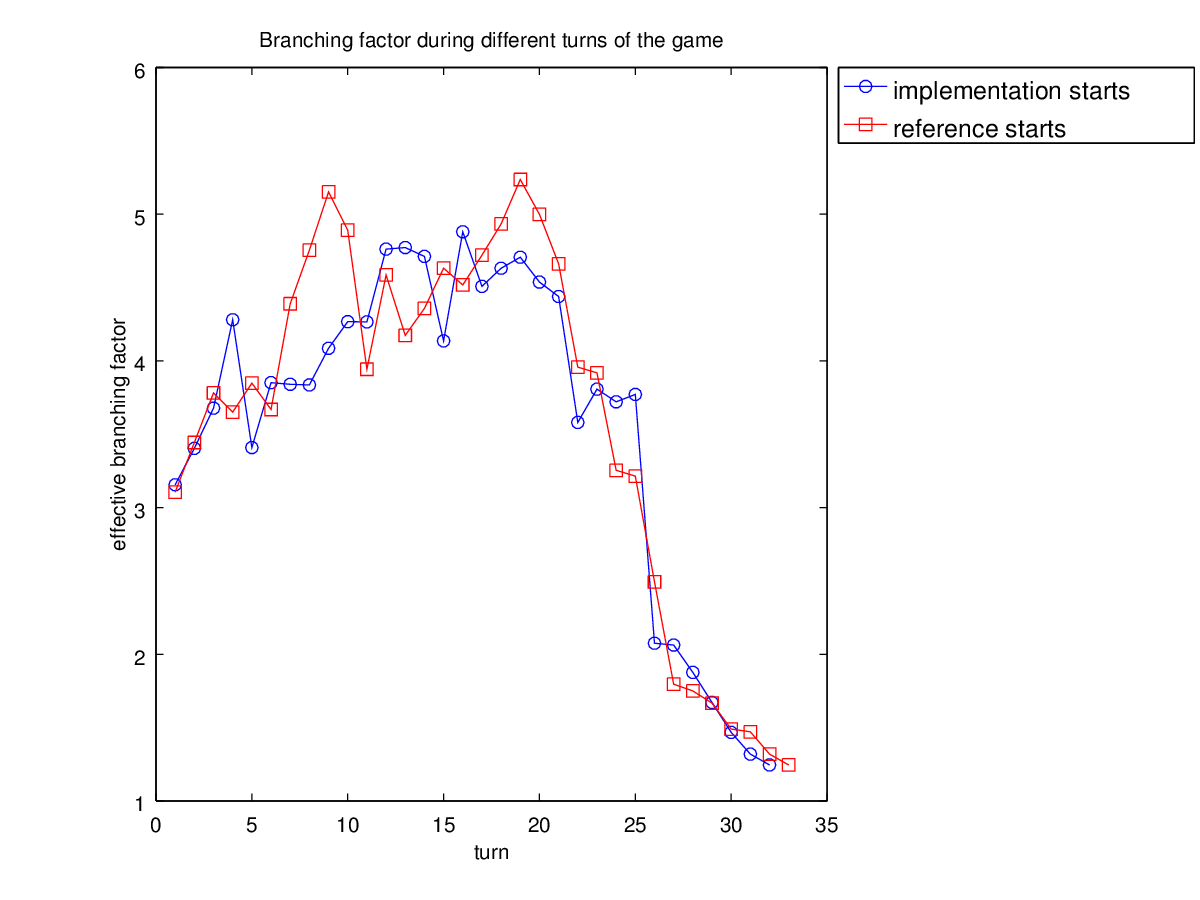
\includegraphics[scale=0.78]{branchingLegend.png}

\caption{Branching factor for each of Leversis turns. It peaks in the middle of the game.} \label{fig:branching}

\end{figure}

\subsection{Time limit}
The problem with the time limit analysis in the previous section is that the last seven (the effective depth) actions are different to the others. Because game over is reached, there is no point in continuing the recursion which then terminates much faster (sometimes below one millisecond as seen in the previous section). The data in table \ref{tab:trimmed} shows statistical properties for the time when the last seven actions in the both games where discarded (the depth until game over is then $14$ or $15$).

\begin{table}

\centering
\begin{tabular}{|l|l|l|l|l|l|l|}
\hline
\textbf{what} & \textbf{mean} & \textbf{median} & \textbf{min} & \textbf{max} & \textbf{<1000} & \textbf{>5000}
\\ \hline
trimmed time (ms) & $2266$ & $2083$ & $952$ & $6212$ & $3.9\%$ & $2.0\%$
\\ \hline
\end{tabular}

\caption{Time data when the last 14 turns of the game are skipped.} \label{tab:trimmed}

\end{table}

There is one outlier taking more than 5 seconds. But otherwise every action is inside the time limit (the second longest taking $4346$ milliseconds). Otherwise the the time used is about usually about two seconds. Considering that the branching factor is about $3.6$, the value seems sound.

If outliers taking more than 5 seconds are totally unacceptable (e.g. due to a special rule), then the approach used in Leversi is insufficient. It should be combined with a time-out, terminating the current recursive call if it has not completed in time and returning the action from the previous iteration. For playing against humans however it is ideal, because the exceptions to the time limit are very few, and it does not waste the players time, by continuing, even though it will not finish in time.

\clearpage

\section{References}
\begin{thebibliography}{99}

\bibitem{aibook} Russel, Stuart; Norvig, Peter. \\
Artificial Intelligence a modern approach \\
Third edition \\
Pearson \\
ISBN-13:	978-0-13-207148-2
ISBN-10:	0-13-207148-7 \\
\copyright 2010 by Pearson Education Inc., publishing as Prentice Hall, Upper Saddle River, New Jersey 07458.

\bibitem{utility} Sannidhanam, Vaishnavi; Annamalai, Muthukaruppan \\
An Analysis of Heuristics in Othello \\
2004 adjusted version \\
Department of Computer Science and Engineering, \\
Paul G. Allen Center, \\
University of Washington, \\
Seattle, WA-98195, \\
\textit{vaishu@cs.washington.edu}, \\
\textit{muthu@cs.washington.edu}.

\end{thebibliography}

\end{document}